% ===========================
%       Chapter 1A.3
%      Carbohydrates:
%     Polysaccharides
%   Created by Michael Tang
%        2024.12.30
% ===========================

\subsubsection{1A.3 Carbohydrates: \underline{Polysaccharides} (多糖)}
\paragraph{Carbohydrates and Energy}
Carbohydrates are a primary source of energy in biological systems, particularly glucose, which is a key monosaccharide used in
cellular respiration.
\begin{itemize}
    \item \textbf{Key Points}
    \begin{itemize}
        \item \textbf{Energy Production:} Glucose ($C_6H_{12}O_6$) is broken down through cellular respiration to produce ATP
        (adenosine triphosphate), which powers cellular activities.
        \item \textbf{End Products:} The breakdown of glucose result in:
        \begin{itemize}
            \item Carbon dioxide ($CO_2$)
            \item Water ($H_2O$)
            \item Large amounts of ATP
        \end{itemize}
        \item \textbf{Glucose Utilization:}
        \begin{itemize}
            \item \textbf{Monosaccharides} such as glucose are rapidly absorbed and used for immediate energy needs.
            \item \textbf{Disaccharides} like sucrose and lactose are broken into monosaccharides for energy production.
            \item \textbf{Polysaccharides} are complex carbohydrates made up of many monosaccharide units joined by glycosidic
            bonds. Note that molecules with between 3 and 10 sugar units are known as \underline{\textbf{oligosaccharides}}
            (低聚糖), while molecules containing 11 or more monosaccharides are known as true polysaccharides.
            \begin{figure}[H]
                \centering
                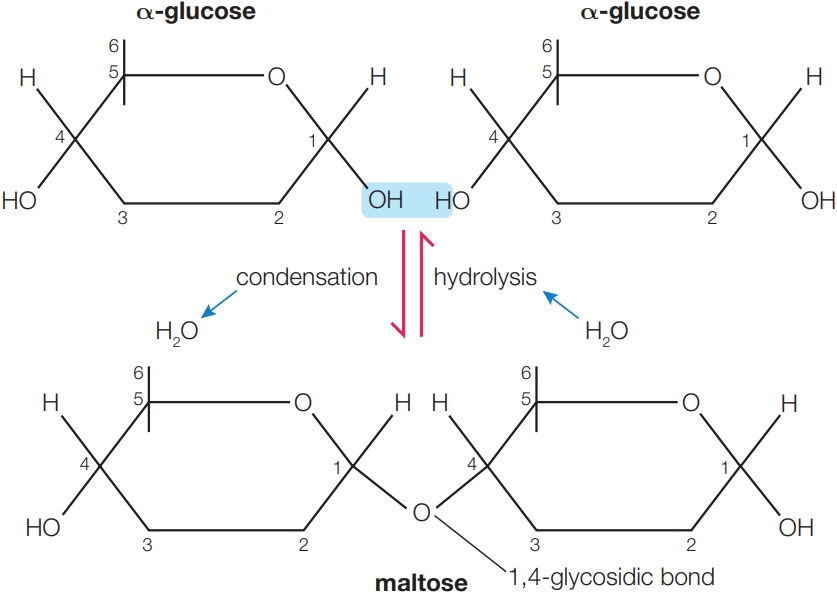
\includegraphics[scale=0.3]{Biology/1A/Images/1A-3-1.png}
                \caption{Glycosidic bonds are made by condensation reactions and broken down by hydrolysis.}
            \end{figure}
            \item \textbf{Exam Hint:} Avoid stating that energy is "created". Instead, describe how chemical energy from glucose
            is transferred to ATP molecules.
        \end{itemize}
    \end{itemize}
    \item \textbf{Properties of Polysaccharides}
    \begin{itemize}
        \item[1.] \textbf{Compact Structure:}
        \begin{itemize}
            \item Takes up little space within cells.
            \item Ideal for storage purposes.
        \end{itemize}
        \item[2.] \textbf{Insolubility:}
        \begin{itemize}
            \item Reduces \underline{osmotic effects} \footnote{\textbf{Osmotic effects:} Osmotic effects refer to the movement
            of water across a \underline{semipermeable membrane} \footnotemark[10] (半透膜) due to differences in solute
            concentration.} (渗透效应) in cells.
            \footnotetext[10]{\textbf{Semipermeable membrane:} It is a membrane that allows certain molecules to pass through
            while blocking others. It permits solvent molecules (such as water) to pass but prevents solute molecules from doing
            so. This property makes semipermeable membranes highly useful in various applications, such as
            \underline{desalination} (海水淡化), where water and salt in seawater are separated using a semipermeable membrane.}
            \item Does not affect water potential.
        \end{itemize} 
        \item[3.] \textbf{Chemical Inactivity:} Does not interfere with cellular reactions.
    \end{itemize}
\end{itemize}
